\documentclass[12pt,letterpaper]{article}
\usepackage[utf8]{inputenc}
\usepackage[spanish]{babel}
\usepackage{graphicx}
\usepackage[left=2cm,right=2cm,top=2cm,bottom=2cm]{geometry}
\usepackage{graphicx} % figuras
% \usepackage{subfigure} % subfiguras
\usepackage{float} % para usar [H]
\usepackage{amsmath}
%\usepackage{txfonts}
\usepackage{stackrel} 
\usepackage{multirow}
\usepackage{enumerate} % enumerados
\renewcommand{\labelitemi}{$-$}
\renewcommand{\labelitemii}{$\cdot$}
% \author{}
% \title{Caratula}
\begin{document}

% Fancy Header and Footer
% \usepackage{fancyhdr}
% \pagestyle{fancy}
% \cfoot{}
% \rfoot{\thepage}
%

% \usepackage[hidelinks]{hyperref} % CREA HYPERVINCULOS EN INDICE

% \author{}
\title{Caratula}

\begin{titlepage}
\begin{center}
\large{UNIVERSIDAD PRIVADA DE TACNA}\\
\vspace*{-0.025in}
\begin{figure}[htb]
\begin{center}

\includegraphics[width=7cm]{./images/logo}
\end{center}
\end{figure}
\vspace*{0.15in}
INGENIERIA DE SISTEMAS  \\

\vspace*{0.3in}
\begin{large}
\textbf{TITULO:} \\
\end{large}

\vspace*{0.1in}
\begin{Large}
\textbf{Informe de Laboratorio 03:Elaborando pruebas
automatizadas de Interfaz de Usuario} \\

\end{Large}

\vspace*{0.3in}
\begin{Large}
\textbf{CURSO:} \\
\end{Large}

\vspace*{0.1in}
\begin{large}
Calidad y Pruebas de Software\\
\end{large}

\vspace*{0.3in}
\begin{Large}
\textbf{DOCENTE:} \\
\end{Large}

\vspace*{0.1in}
\begin{large}
 Ing. Patrick Cuadros Quiroga\\
\end{large}

\vspace*{0.4in}
\vspace*{0.1in}
\begin{large}
\textbf{INTEGRANTES:} \\
\begin{flushleft}
Yaneth Virginia Aquino Huallpa \hfill	(2017059286)\\

\centering  %CENTRA UN TEXTO
\vspace*{0.9in}
\begin{large}
Tacna
\end{large}

\end{flushleft}
\end{large}
\end{center}

\end{titlepage}


\tableofcontents % INDICE
\thispagestyle{empty} % INDICE SIN NUMERO
\newpage
\setcounter{page}{1} % REINICIAR CONTADOR DE PAGINAS DESPUES DEL INDICE


\section{Crear una aplicación WPF} 
\begin{itemize}
 \item  Cree un proyecto Aplicación de WPF (.NET Framework) y asígnele el nombre SimpleWPFApp.
\item Se abre WPF Designer y se muestra la MainWindow del proyecto.
\begin{center}
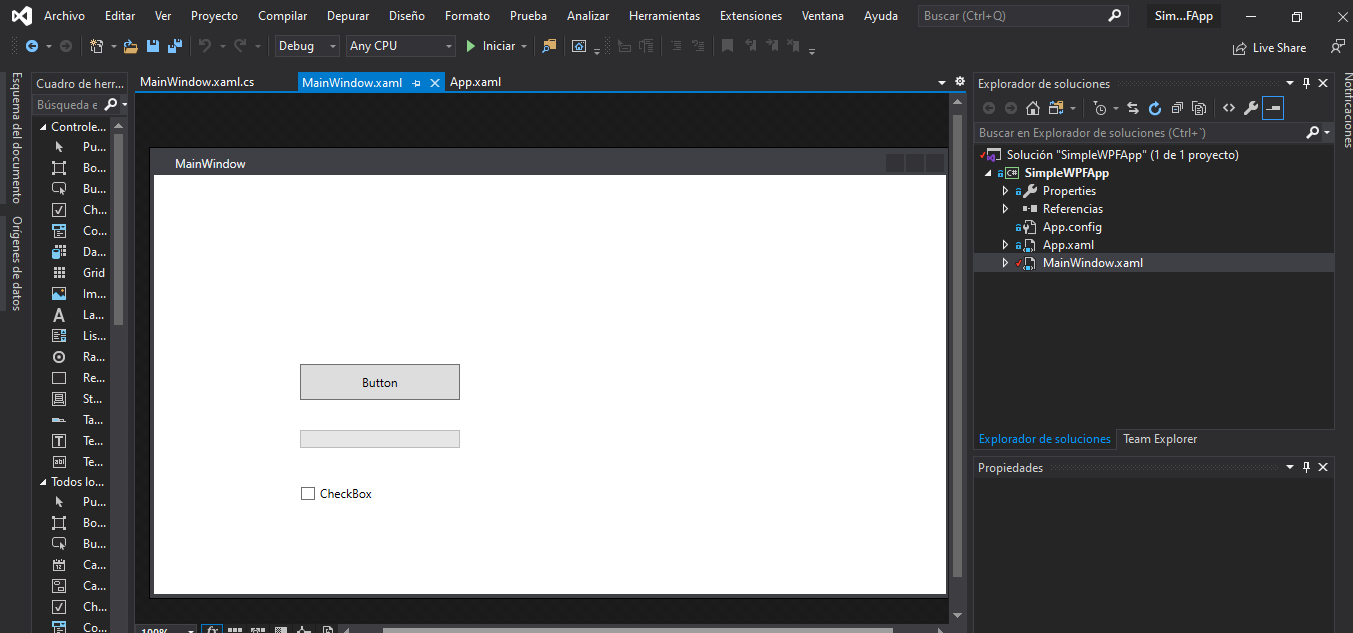
\includegraphics[width=\columnwidth]{images/1}\newline
\end{center}
\item MainWindow.xmal.cs se muestra en el Editor de código con el cursor en el nuevo método button1 Click.En la parte superior de la clase MainWindow, agregue un delegado. El delegado se utilizará para la
barra de progreso. Para agregar el delegado, agregue el código siguiente:
\begin{center}
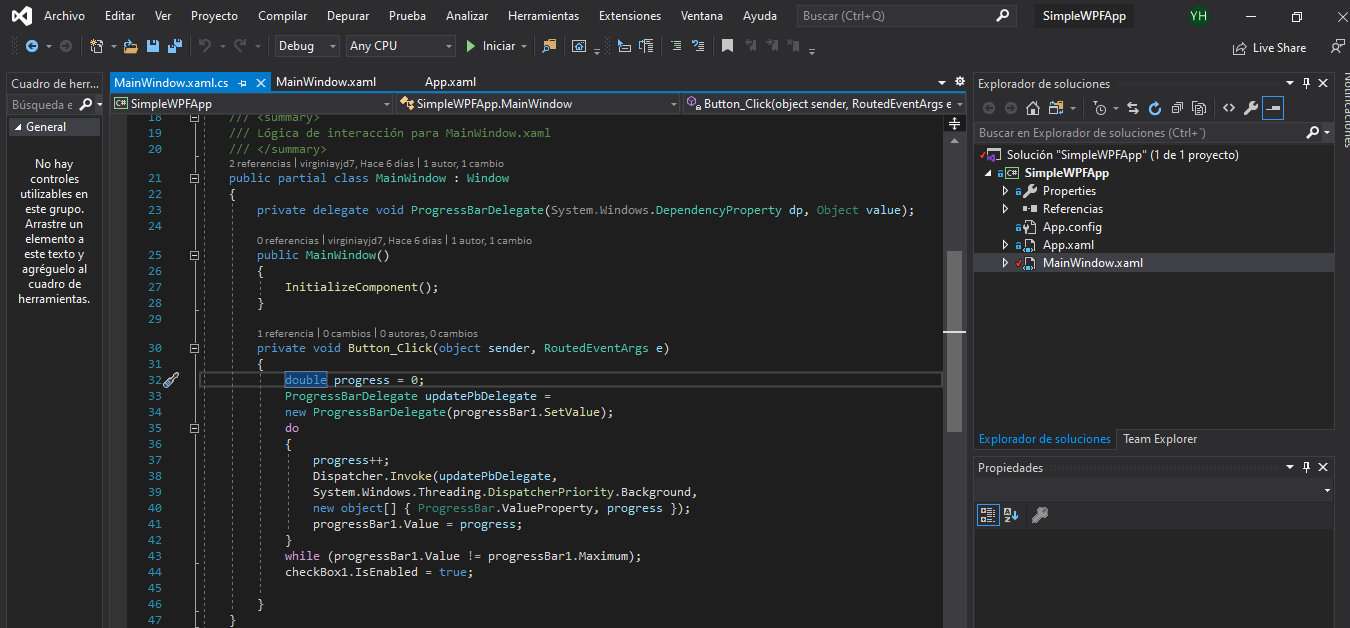
\includegraphics[width=\columnwidth]{images/2}\newline
\end{center}
\item Ejecutar la aplicación WPF
\begin{center}
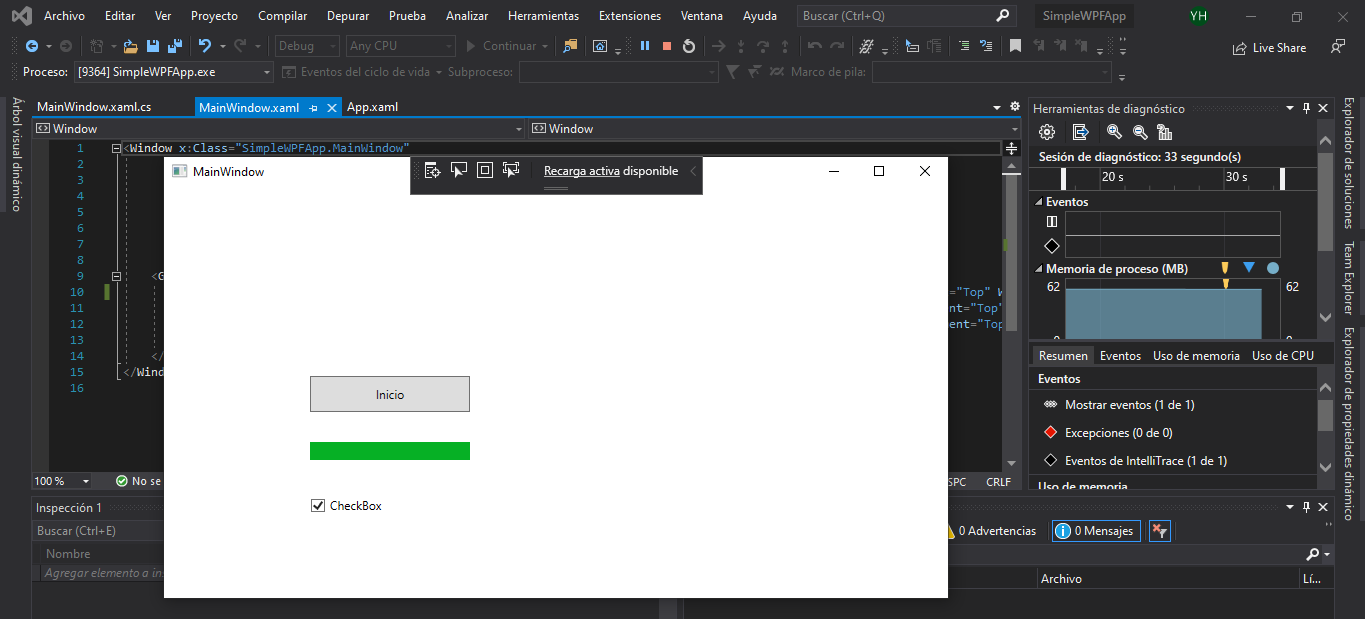
\includegraphics[width=\columnwidth]{images/3}\newline
\end{center}
\end{itemize}
\section{Crear un acceso directo a la aplicación de WPF:} 

\begin{itemize}
\item Busque la aplicación SimpleWPFApp que creó anteriormente.Cree un acceso directo en el escritorio a la aplicación SimpleWPFApp.
\begin{center}
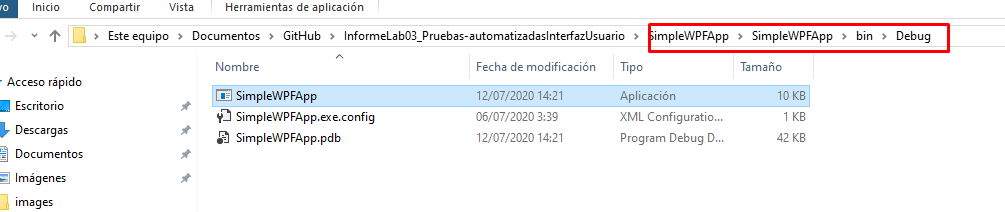
\includegraphics[width=\columnwidth]{images/4}\newline
\end{center} \item Haga clic con el botón derecho en SimpleWPFApp.exe y elija Copiar. En el escritorio, haga clic con el botón derecho y elija Pegar acceso directo.
\begin{center}
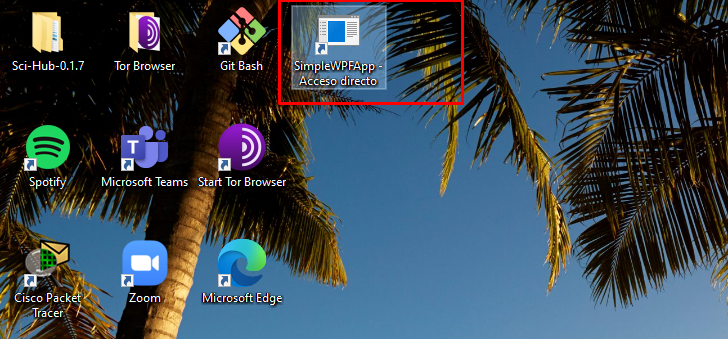
\includegraphics[width=\columnwidth]{images/5}\newline
\end{center}
\end{itemize}
\section{Crear una prueba automatizada de IU para SimpleWPFApp} 
\begin{itemize}
\item En el Explorador de soluciones, haga clic con el botón derecho en la solución y
elija Agregar > Nuevo proyecto.Busque la plantilla de proyecto Proyecto de prueba automatizada de IU, selecciónela y siga los pasos
hasta que se cree el proyecto.
\begin{center}
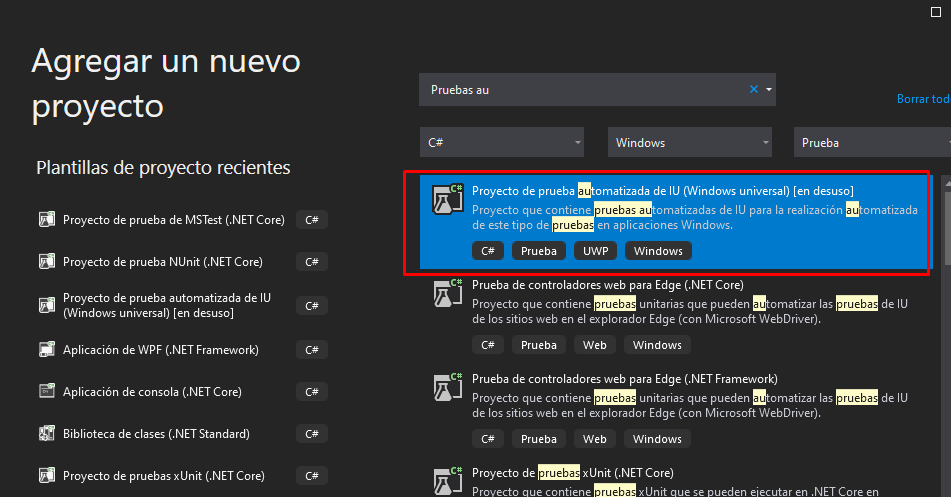
\includegraphics[width=\columnwidth]{images/6}\newline
\end{center}
 \item El nuevo proyecto de prueba automatizada de IU, CodedUITestProject1
\begin{center}
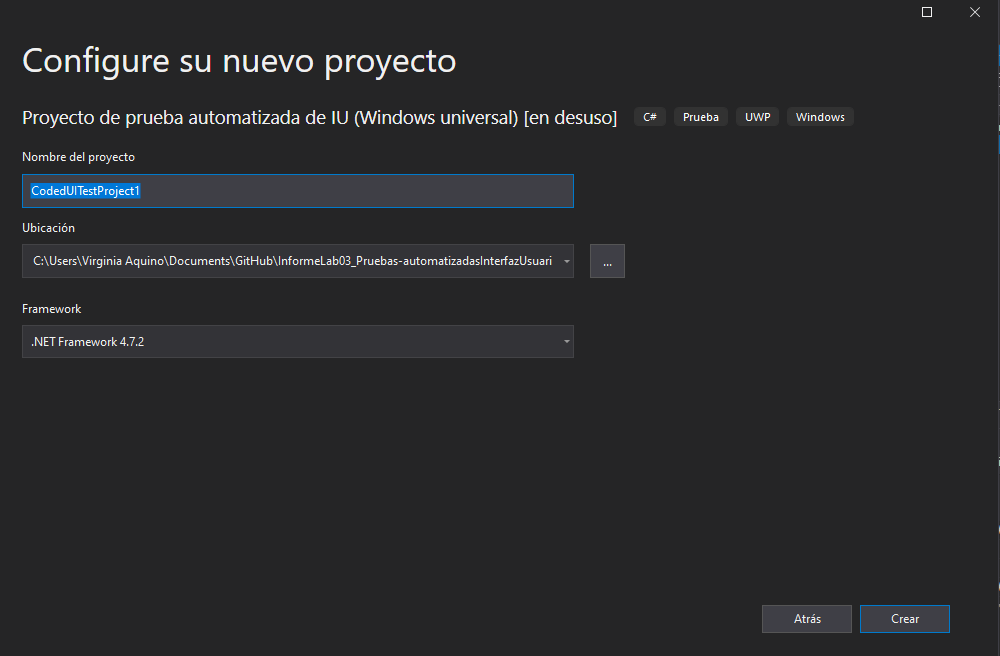
\includegraphics[width=\columnwidth]{images/7}\newline
\end{center}
\item se agrega a la solución y se abre el cuadro de diálogo Generar código para prueba automatizada de IU.
\begin{center}
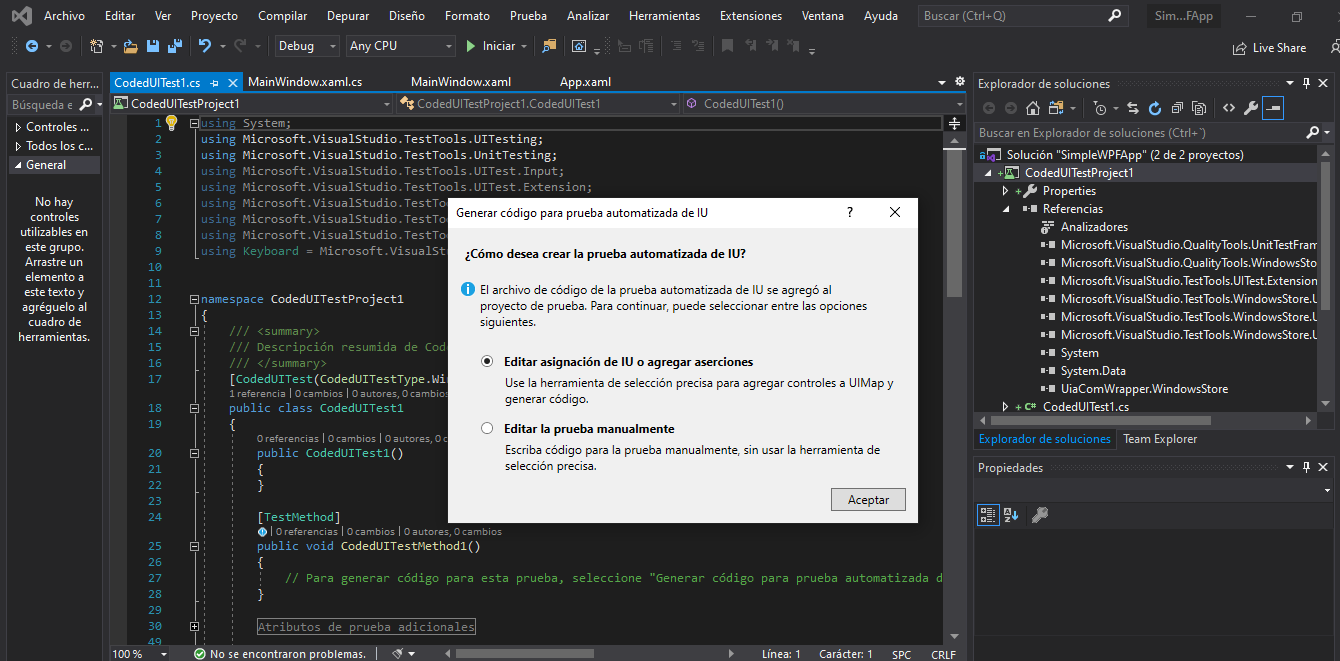
\includegraphics[width=\columnwidth]{images/8}\newline
\end{center}
\end{itemize}

\end{document}